

\section{The Families to Persons Benchmark}
\label{sec:FamiliesToPersons}

\NOTE{\emph{Length:} 2 p., \emph{Resonsible:} Bernhard}

%\NOTE{Based on TTC 2017, Section~2, or ENASE 2018, Section~3. Metamodels, functionality of batch and incremental transformations, challenges. Presentation of test cases, classified according to the developed taxonomy.}

\noindent As mentioned, different variants of the Families to Persons case have been proposed in the literature. Below, we will present the TTC 2017 variant of the case, mainly following  \cite{Anjorin2017a} and \cite{ENASE2018-Westfechtel}, in the terminology of model-driven software development, even though tools solving the case are not required to be model-driven. 

\begin{figure}[tb!]
	\centering
	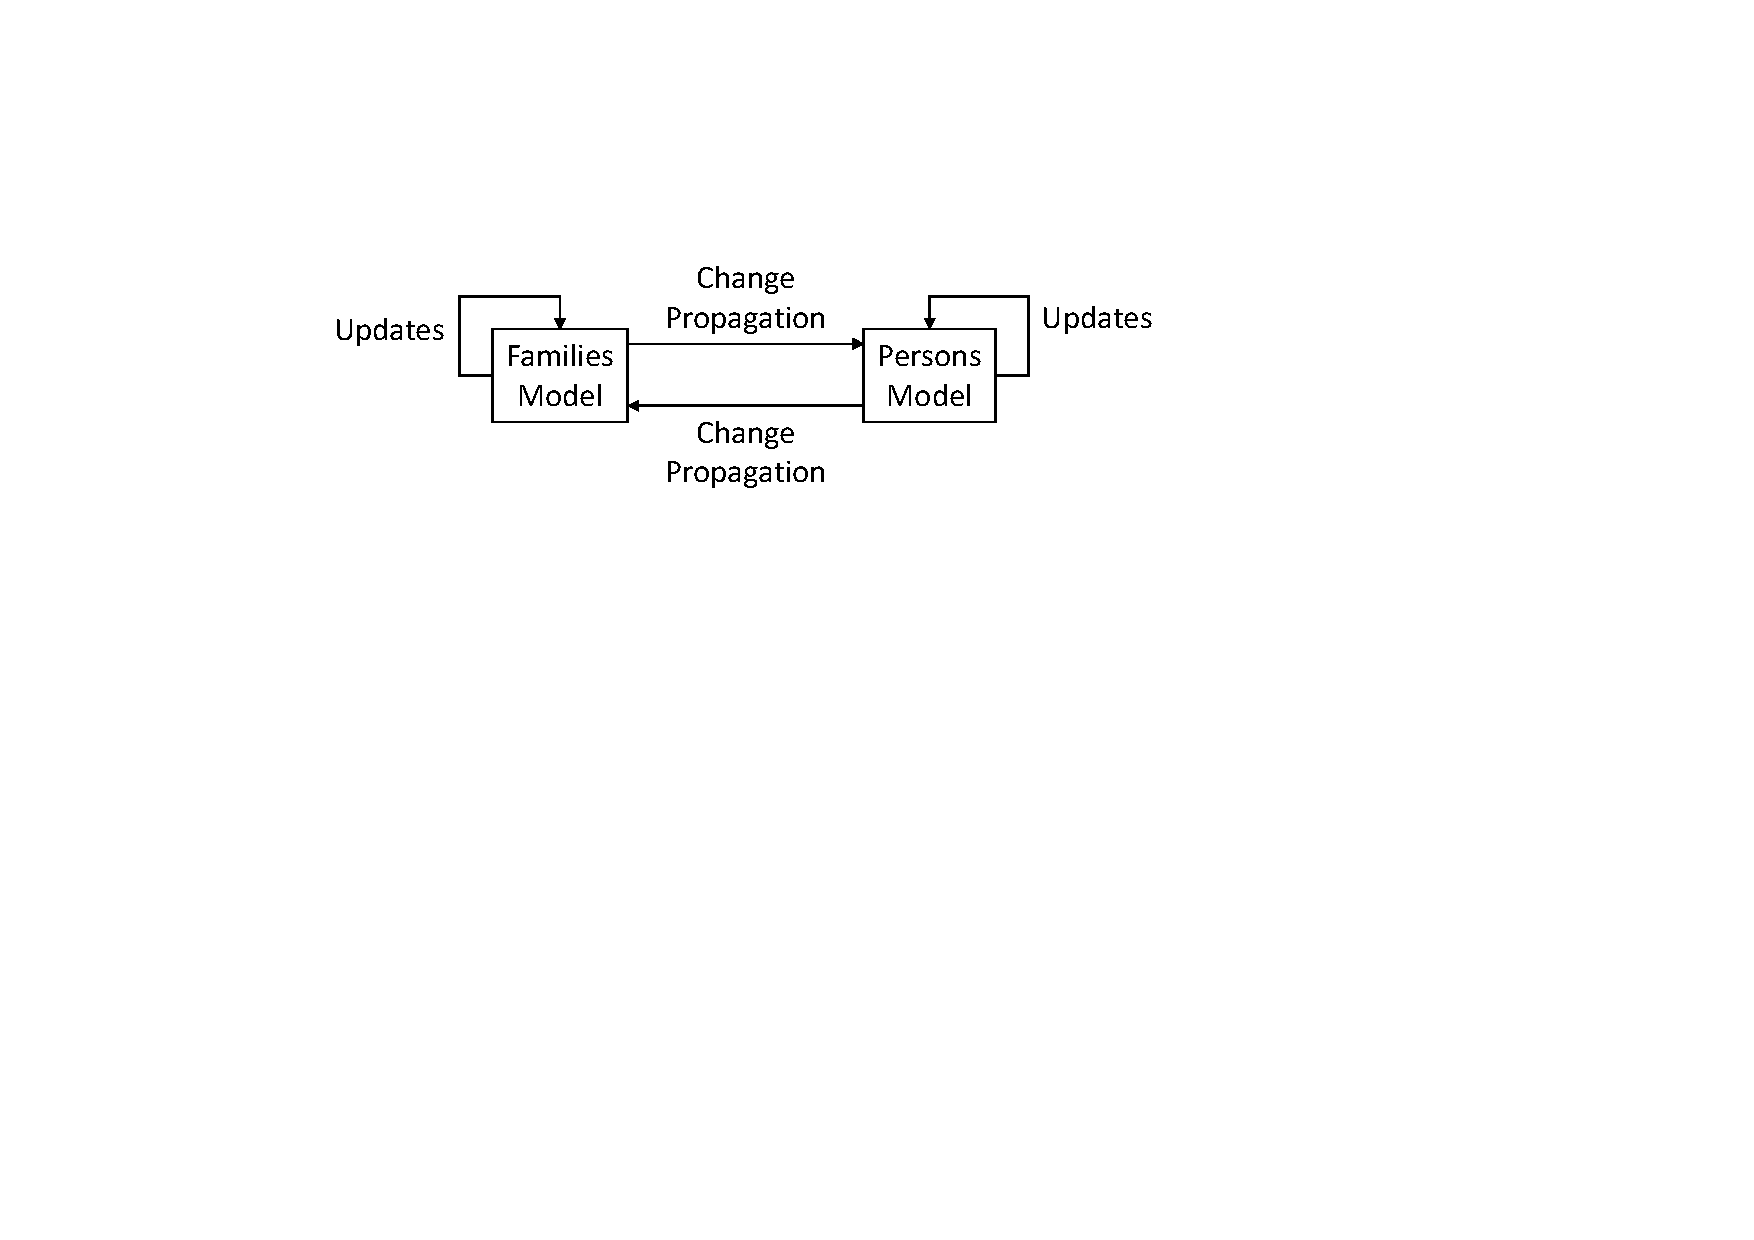
\includegraphics[width=0.8\columnwidth]{diagrams/Families2PersonsCase}
	\caption{The Families to Persons case}
	\label{fig:case}
\end{figure}

In the Families to Persons case, two related, but differently structured models have to be kept consistent (Figure~\ref{fig:case}): A \emph{families model} with parents and children, and a \emph{persons model} containing a flat set of males and females. Updates may be performed on both models, and have to be propagated in both directions. Neither model is a view of its opposite; information loss may occur in both transformation directions.

\subsection{Metamodels and Consistency}
\label{sec:MetamodelsAndConsistency}

For metamodeling, we employ \emph{Ecore} --- an implementation of Essential MOF, a subset of MOF \cite{MOF-2.5.1}, provided by the Eclipse Modeling Framework \cite{steinberg09}. Please note that we adopt the following terminology: A \emph{model} represents a collection of instance data. A \emph{metamodel} is a ``model for models" and defines the types of objects, attributes, and links, as well as the rules for their composition. When implementing the benchmark in a bx tool, the metamodel displayed in Figure~\ref{fig:metamodels} may be reused as it stands, or it may be represented in a different --- yet equivalent --- way (e.g., type definitions in a functional programming language, as done in BiGUL).

\begin{figure}[tb!]
	\centering
	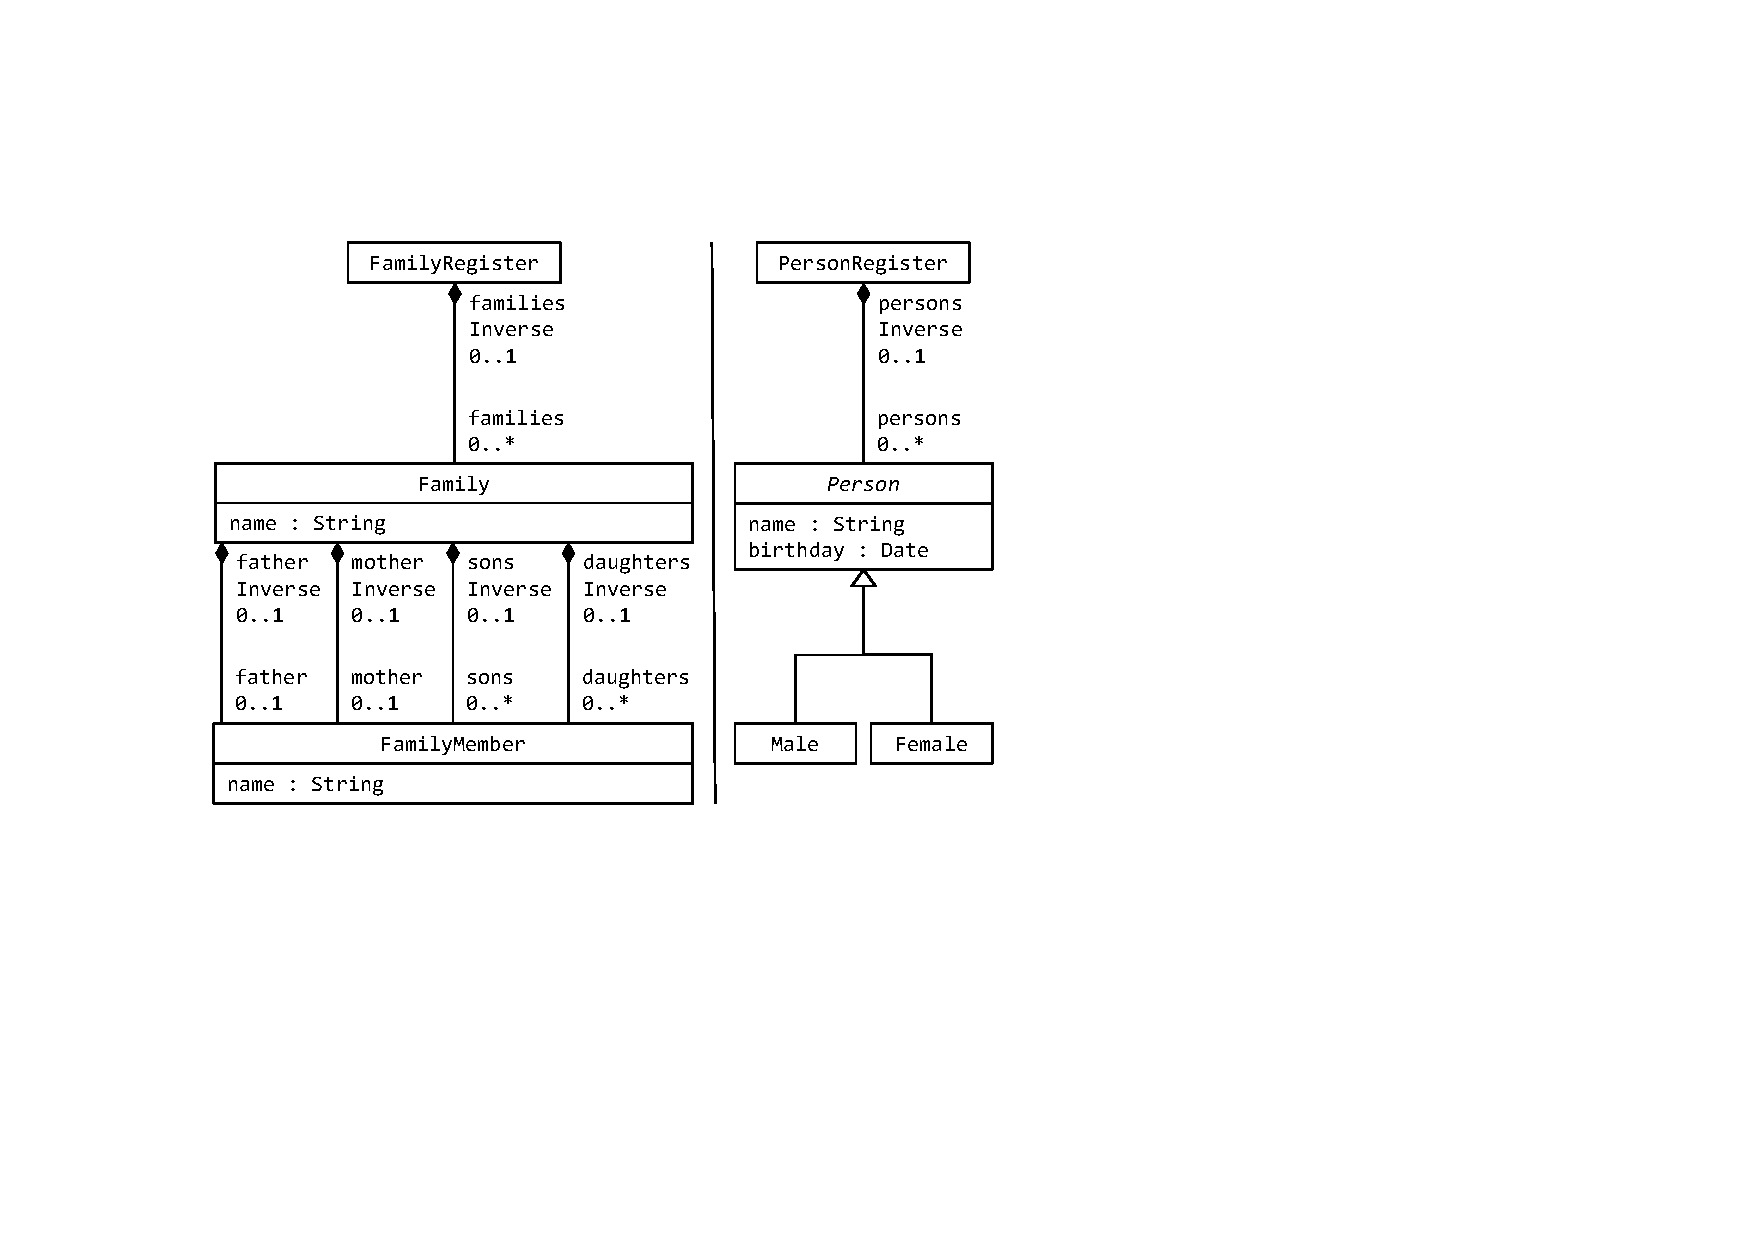
\includegraphics[width=\columnwidth]{diagrams/Metamodels}
	\caption{Metamodels}
	\label{fig:metamodels}
\end{figure}

\begin{figure*}[tb!]
	\centering
	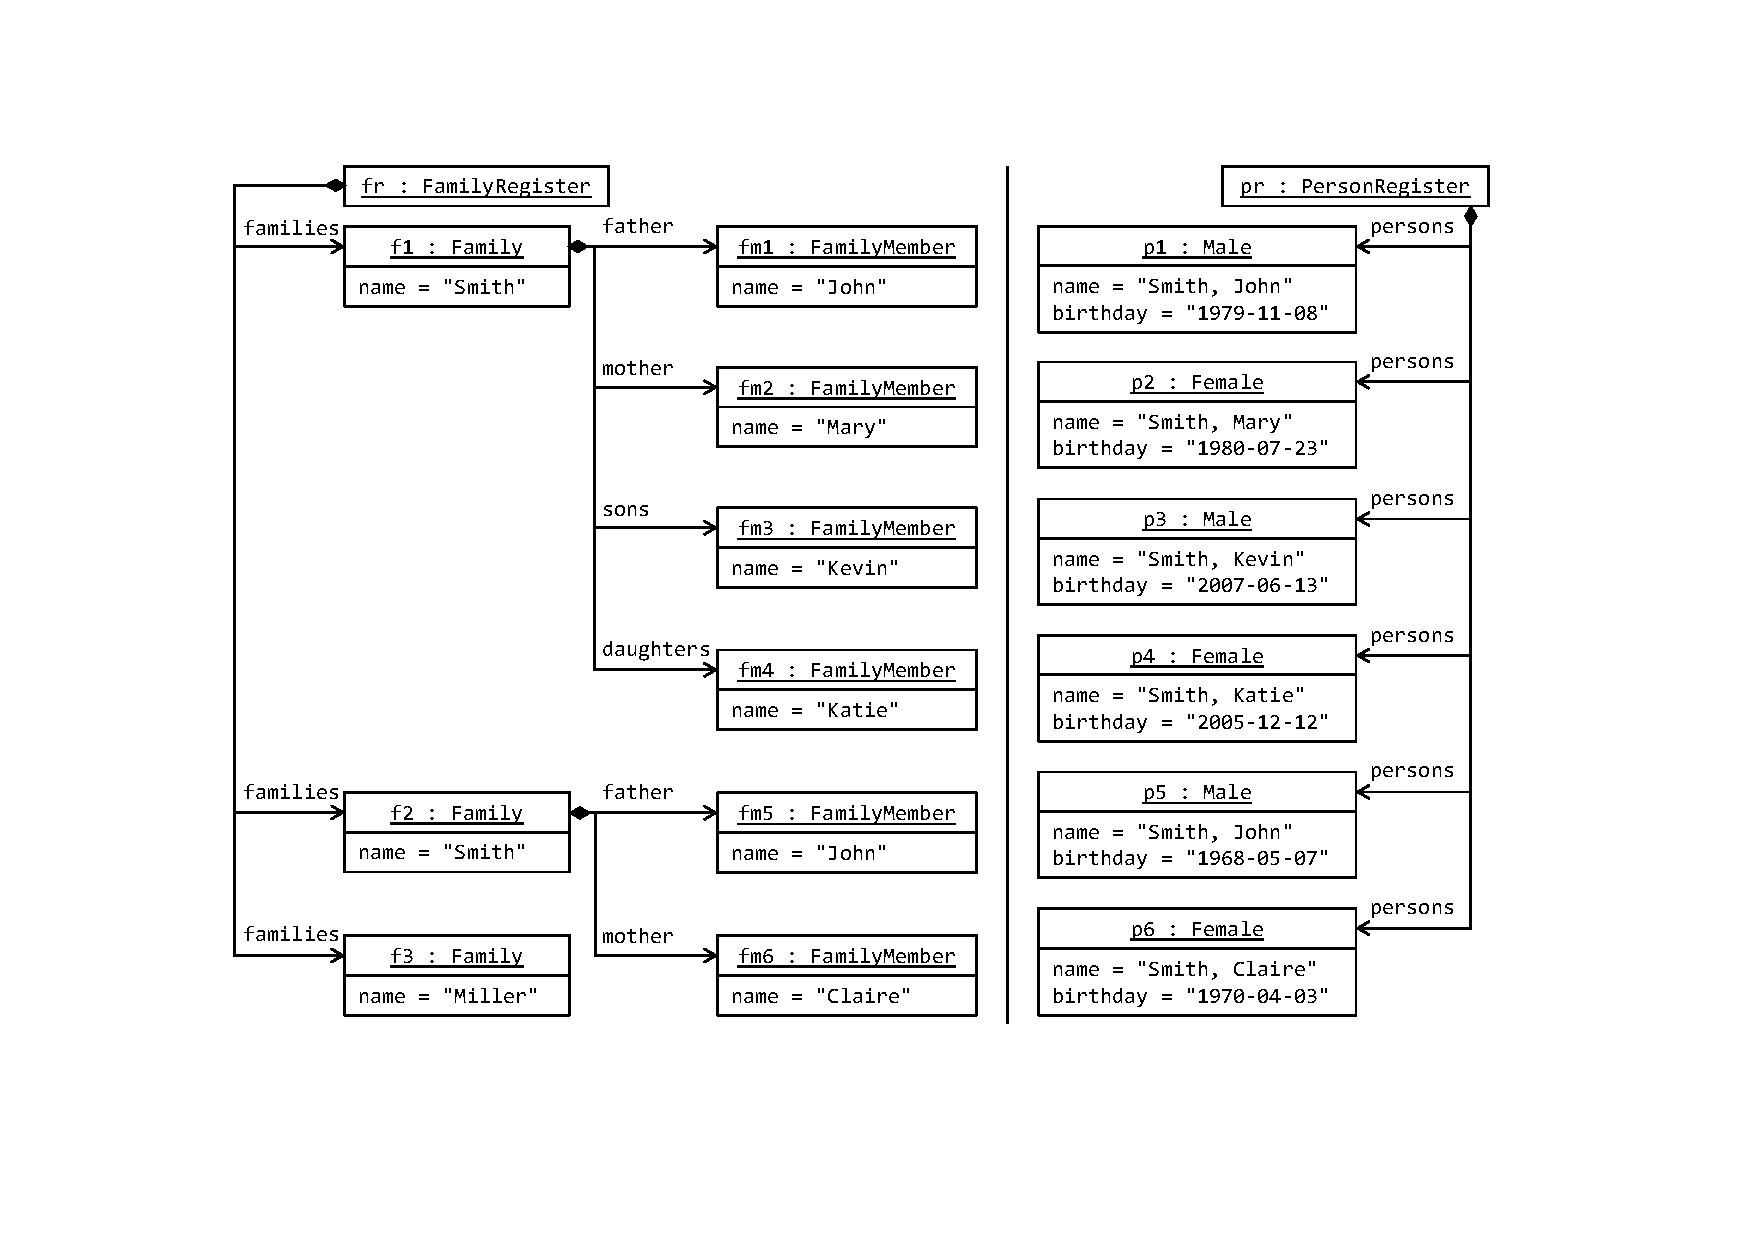
\includegraphics[width=0.75\textwidth]{diagrams/Models}
	\caption{Example of mutually consistent models}
	\label{fig:models}
\end{figure*}

We assume a unique root in each model. A family register stores an unordered collection of families. Each family has members who are distinguished by their roles. The metamodel permits at most one mother and at most one father as well as an arbitrary number of daughters and sons. A person register maintains a flat unordered collection of persons who have a birthday and are either male or female. Note that key properties may be assumed in neither model: There may be multiple families with the same name, name clashes are even allowed within a single family, and there may be multiple persons with the same name and birthday. 

A families model is \emph{consistent} with a persons model if a bijective mapping between family members and persons can be established such that the following conditions hold:

\begin{enumerate}
	\item  Mothers and daughters (fathers and sons) are paired with females (males).
	\item  The name of every person $p$ is ``$f.name$,~$m.name$'', where $m$ is the member (in family $f$) paired with $p$.
\end{enumerate}

An example of mutually consistent models, conforming to the metamodel of Figure~\ref{fig:metamodels}, is given in Figure~\ref{fig:models}. Birthday attributes in the persons model are omitted because they are not relevant for the consistency relation.



\subsection{Batch Transformations}
\label{sec:BatchTransformations}

After running a transformation in any direction, it is required that the participating models are mutually consistent according the definition given above. However, this requirement does not suffice to define the functionality of transformations in a unique way. Below, we first consider \emph{batch transformations}, where the target model is created from scratch.

The functionality of a \emph{forward transformation} may be defined in a straightforward way: Map each family member to a person of the same gender and compose the person's name from the family name and the first name; the birthday remains unset because no data are stored in the families model from which birthdays could be inferred. This transformation is deterministic (but not injective). When applied to the families model on the left-hand side of Figure~\ref{fig:models}, it returns the persons model on the right-hand side. 

The \emph{backward transformation} is more involved: A person may be mapped either to a parent or a child, and persons may be grouped into families in different ways. The consistency relation is \emph{non-deterministic}: For a given persons model, there are multiple families models which satisfy the consistency relation. As a consequence, there are different options to define the behavior of the backward transformation.

We decided to require a \emph{configurable} backward transformation, which is controlled by two Boolean parameters: \code{prefer\-Parent\-To\-Child} defines whether a person is mapped to a parent or a child. \code{prefer\-Existing\-To\-New\-Family} determines whether a person is added to an existing family (if available), or a new family  is created along with a single family member. If both parameters are set to true, the second parameter takes precedence: If a family is available with a matching family name, but there is no matching family with an unoccupied parent role, the member is inserted into an existing family as a child.

%Please notice that the configuration parameters reduce non-determinism without eliminating it completely. If  both configuration parameters are set to true, the resulting families model depends on the order in which persons are processed. For example, in Figure~\ref{fig:models}, there are three candidates for the father role in the Smith family (recall that the collection of persons is unordered). 

 
\subsection{Incremental Transformations}
\label{sec:IncrementalTransformations}

For \emph{incremental transformations}, updates such as insertions, deletions, changes of attribute values, and move operations have to be considered. In \emph{forward direction}, insertion of a family has no effect on the target model. Insertion of a member results in insertion of a corresponding person; likewise for deletions. If a family is deleted, all persons corresponding to its members are deleted. If a member is renamed, the corresponding person is renamed accordingly. If a family is renamed, all persons corresponding to family members are renamed. If a member is moved, different cases have to be distinguished. If the gender is retained, the corresponding person object is preserved; otherwise, it is deleted, and a new person object with a different gender is created whose attributes are copied from the old person object. A local move within a family does not affect the corresponding person's name; a move to another family results in a potential update of the person's name. 

In \emph{backward direction}, the effect of an update depends on the values of the configuration parameters which may vary between different transformation executions. Please note that the parameter settings must not affect already established correspondences; rather, they apply only to future updates. Deletion of a person propagates to the corresponding family member. If a person is inserted, it depends on the configuration parameters how insertion propagates to the families model (see above). Persons cannot be moved because the persons model consists of a single, flat, and unordered collection. Changes of birthdays do not propagate to the opposite model. If the first name of a person is changed, the first name of the corresponding family member is updated accordingly. Finally, if the family name of a person is changed, this change does not affect the current family and its members: The family preserves its name even if it does not contain other members; thus, the update has no side effects on the existing family. Rather, the corresponding family member is moved to another family, which may have to be created before the move; the precise update behavior depends on the parameter settings.

\subsection{Transformation Laws}
\label{sec:TranformationLaws}

\NOTE{Maybe this subsection is obsolete. As it stands, there are some problems with definitions. Here, correctness merely requires that the consistency relation holds after an update propagation; in Section~1, this notion was used with reference to the test cases. Furthermore, the round-trip laws are not stated precisely. The cited reference refers to the view-update scenario, which is not applicable here. Anyway: This subsection should be retained only if the laws are defined precisely  in Section~3; then, it should be re-aligned with Section~3.}

\noindent The transformations developed for the Families to Persons benchmark should satisfy a set of general \emph{laws} \cite{SOSYM-Stevens2010}. First, the result of a transformation from $s$ to $t$ should be \emph{correct}, i.e., $s$ and $t$ should be mutually consistent (see Section~\ref{sec:MetamodelsAndConsistency}). Furthermore, transformations should be \emph{hippocratic}: The target model should not be changed if consistency has already been established. Thus, an immediate re-run of a transformation establishing correctness should have no effect (even if configuration paramaters are switched in the backward transformation). Finally, \emph{round-trip laws} \cite{TOPLAS2007-Foster} should be satisfied: A backward transformation immediately following a forward transformation should leave the original source model untouched; likewise for a forward transformation following a backward transformation.

\subsection{Challenges}
\label{sec:Challenges}

The Families to Persons case includes a number of \emph{challenges} which are summarized below:

\begin{description}
	\item[\textbf{Heterogeneous metamodels}] The transformation has to perform a mapping between heterogeneous metamodels, where the same information is represented in different ways (concerning e.g.\ names and genders).
	\item[\textbf{Loss of information}] The family structure is lost in the forward transformation; birthdays are lost in the backward transformation.
	\item[\textbf{No keys}] There are no uniquely identifying properties for family members or persons, which makes propagation of changes difficult.
	\item[\textbf{Non-determinism}] The consistency relation is non-deterministic: For a given families model, there are multiple persons models satisfying the consistency relation (since birthdays may be arbitrarily selected). Likewise, for a given persons model there are multiple families models being consistent with the persons model (due to different groupings into families and different roles in these families)
	\item[\textbf{Configurability}] The behavior of the backward transformation is controlled by configuration parameters for determining roles of persons and groupings of persons into families. Parameters may be changed from execution to execution and should affect only new elements of the persons model in each run.
	\item[\textbf{Renamings and moves}] Changes to be propagated include not only creations and deletions, but also renamings and moves, which must not be reduced to deletions and creations (otherwise, the principle of \emph{least change} \cite{SOSYM-Macedo2016}, which demands that the changes are propagated in a minimally invasive way, would be violated). 
	\item[\textbf{Order-dependent update behavior}] The backward transformation depends on the order in which change operations on the persons model are processed. For example, if two persons are to be inserted into the same family as parents, the first one will be inserted as parent, and the second one will follow as a child.
	\item[\textbf{Specific requirements to change operations}] The\\ case description includes specific requirements to change operations. For example, if the family name of a person is changed, the person should be moved to another family (rather than having the family name updated, with side effects on other members). 
\end{description}
